%%%%%%%%%%%%%%%%%%%%%%%%%%%%%%%%%%%%%%%%%
% baposter Portrait Poster
% LaTeX Template
% Version 1.0 (15/5/13)
%
% Created by:
% Brian Amberg (baposter@brian-amberg.de)
%
% This template has been downloaded from:
% http://www.LaTeXTemplates.com
%
% License:
% CC BY-NC-SA 3.0 (http://creativecommons.org/licenses/by-nc-sa/3.0/)
%
%%%%%%%%%%%%%%%%%%%%%%%%%%%%%%%%%%%%%%%%%

%----------------------------------------------------------------------------------------
%	PACKAGES AND OTHER DOCUMENT CONFIGURATIONS
%----------------------------------------------------------------------------------------

\documentclass[a0paper,portrait]{baposter}
\usepackage{cite,url,amsthm,footmisc,bm}
\usepackage{amsmath,graphicx,amssymb,algorithm,algorithmic,graphicx,subfigure,epsfig,multirow,threeparttable,booktabs,bm,mathdots,tabularx}
\usepackage[font=large,labelfont=bf]{caption} % Required for specifying captions to tables and figures
\usepackage{booktabs} % Horizontal rules in tables
% \usepackage{relsize} % Used for making text smaller in some places

\graphicspath{{figures/}} % Directory in which figures are stored

\definecolor{bordercol}{RGB}{40,40,40} % Border color of content boxes
\definecolor{headercol1}{RGB}{186,215,230} % Background color for the header in the content boxes (left side)
\definecolor{headercol2}{RGB}{80,80,80} % Background color for the header in the content boxes (right side)
\definecolor{headerfontcol}{RGB}{256,256,256} % Text color for the header text in the content boxes
\definecolor{boxcolor}{RGB}{256,256,256} % Background color for the content in the content boxes

\begin{document}

\background{ % Set the background to an image (background.pdf)
\begin{tikzpicture}[remember picture,overlay]
\draw (current page.north west)+(-2em,2em) node[anchor=north west]
{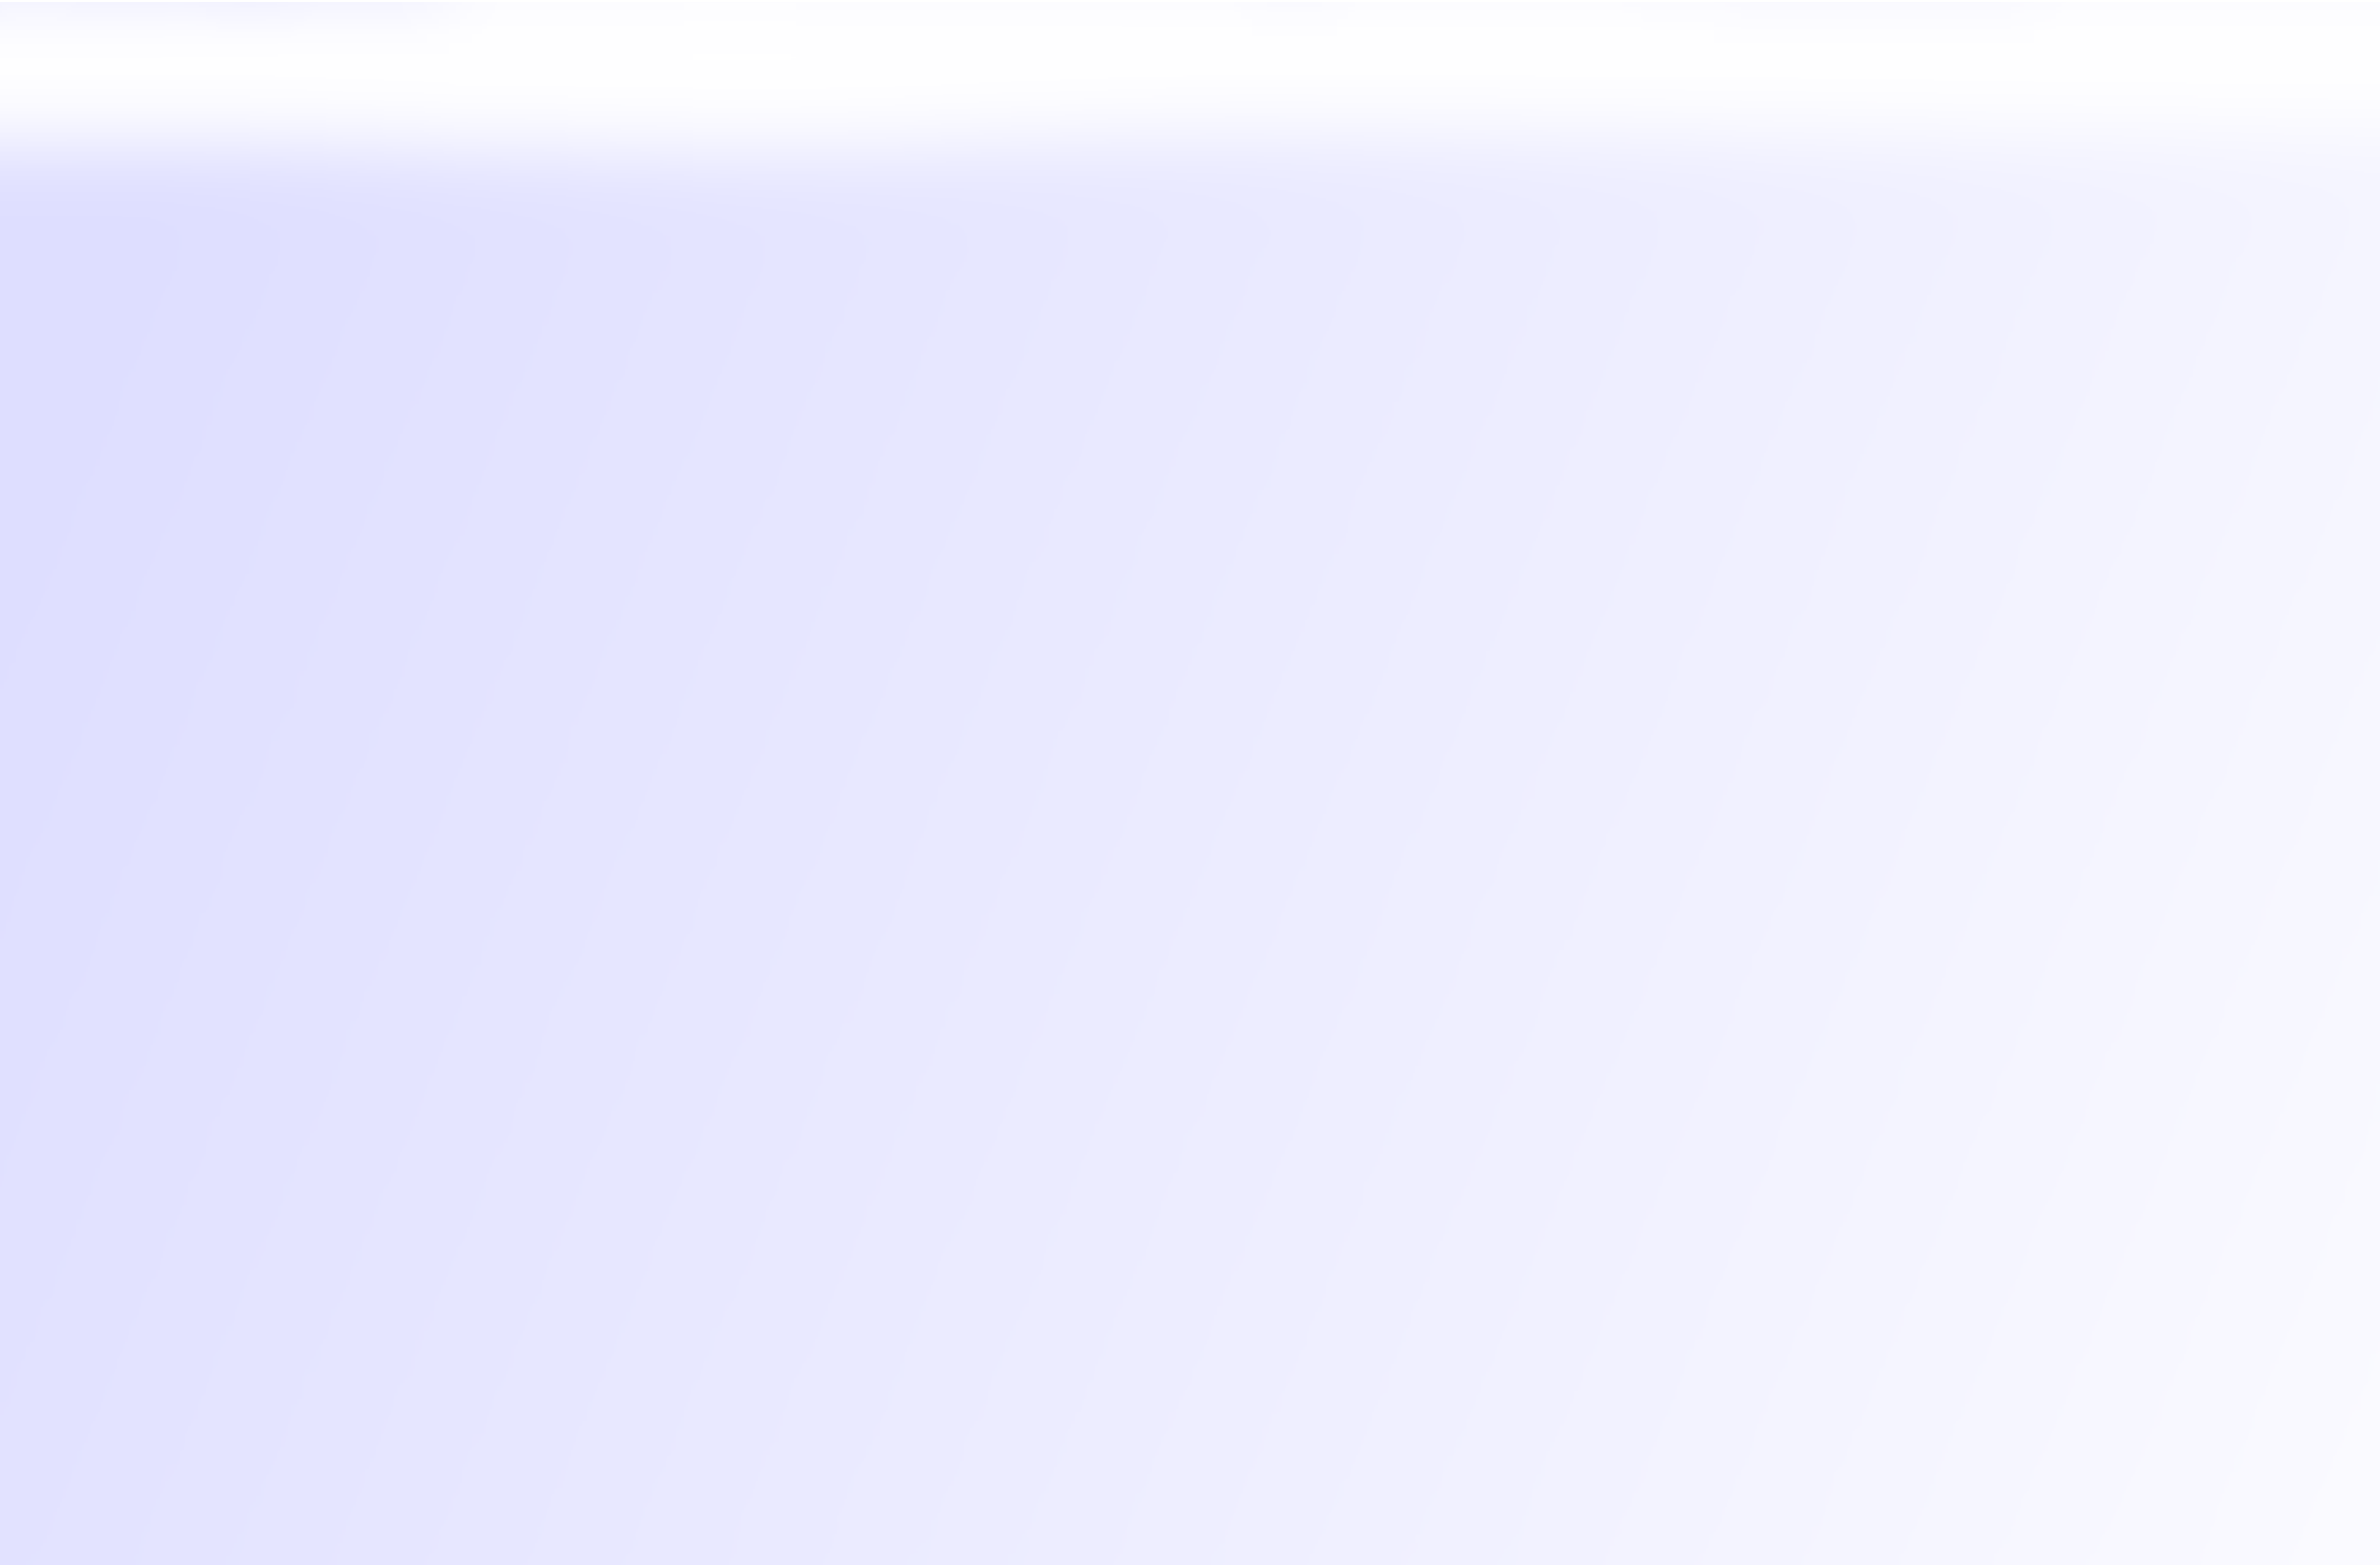
\includegraphics[height=1.1\textheight]{background}};
\end{tikzpicture}
}

\begin{poster}{
grid=false,
borderColor=bordercol, % Border color of content boxes
headerColorOne=headercol2, % Background color for the header in the content boxes (left side)
headerColorTwo=headercol1, % Background color for the header in the content boxes (right side)
headerFontColor=headerfontcol, % Text color for the header text in the content boxes
boxColorOne=boxcolor, % Background color for the content in the content boxes
headershape=roundedright, % Specify the rounded corner in the content box headers
headerfont=\Large\sf\bf, % Font modifiers for the text in the content box headers
textborder=rectangle,
background=user,
headerborder=open, % Change to closed for a line under the content box headers
boxshade=plain
}
{}
%
%----------------------------------------------------------------------------------------
%	TITLE AND AUTHOR NAME
%----------------------------------------------------------------------------------------
%
{\bf SCANNING THE INTERNET FOR VULNERABLE DEVICES} % Poster title
{\vspace{1em} Anna Sim and Sean Wang\\} % Author names
% {\smaller ahs996@utexas.edu}} % Author email addresses
% {
\includegraphics[scale=1.55]{logo}} % University/lab logo

%----------------------------------------------------------------------------------------
%	ABSTRACT
%----------------------------------------------------------------------------------------

\headerbox{Abstract}{name=introduction,column=0,row=0}{
\begin{large}
Shodan is a popular search engine used to detect Internet-facing devices by performing port scans on a network.
By using this tool, we are able to collect data from IPs across the
Internet, focusing on select vulnerabilities. In this paper, we will
discuss how Shodan is used to find numbers of remote machines on the Internet
that are vulnerable from selected CVEs. The data
is then analyzed to see what the detected machines have in common.
After recording data from Shodan, we then created our own scanner to scan the Internet for vulnerable
machines on the same ports as those of the identified devices in the CVEs.
The results are then compared to those of Shodan's scan.

\end{large}
}

%----------------------------------------------------------------------------------------
%	MATERIALS AND METHODS
%----------------------------------------------------------------------------------------

\headerbox{Methods}{name=methods,column=0,below=introduction}{

\begin{Large}
We are analyzing for vulnerable devices from three CVEs using
Shodan and our custom scanning tool. The CVEs listed below were chosen due 
to their commonality, since there would be more 
information to work with for a better comparison  between the two scanning methods.
\begin{enumerate}
    \item{CVE-2014-2256 \cite{CVE-2014-2256}: On Shodan,
search term used to find these vulnerable devices is: \verb|siemens port:"102"|
Our custom tool performs a scan on port 102 and returns a list of probed devices. }
\end{enumerate}


For CVE-2019-0708, which is described as a remote code execution vulnerability that
exists in Microsoft's Remote Desktop Protocol in Windows\cite{CVE-2019-0708}, we search for devices with port 3389 open and running versions of 
Windows in Shodan. We search for
the term \verb|port:"3389"| with one of the following: \verb|os:"Windows 7 or 8"|,
\verb|os:"Windows XP"|, \verb|2003|, or \verb|2008|. In this case, the last two
terms refer to versions of Windows Server. 

Finally, CVE-2018-0101 is a vulnerability in Cisco's Adaptive Security Appliance (ASA)
Software, specifically the Secure Sockets Layer (SSL) VPN functionality. In Shodan,
we use the search term \verb|"Set-Cookie: webvpn=;" ssl:"ASA Temporary"|
% what our custom tool scan is

\end{Large}
}

%----------------------------------------------------------------------------------------
%	CONCLUSION
%----------------------------------------------------------------------------------------

\headerbox{Conclusion}{name=conclusion,column=0,below=methods}{

In this paper, we proposed a novel GUFS method, termed JGUFS, which simultaneously performs graph construction and feature selection. Instead of performing feature selection on a fixed graph, JGUFS successfully avoided the disadvantages caused by the two-stage strategy. In JGUFS, the subobjectives respectively corresponding to graph construction and unsupervised feature selection could co-evolve towards the optimum. An efficient iterative optimization method with convergence guarantee was presented to optimize the JGUFS objective. Extensive experiments were conducted on representative data sets to demonstrate the excellent performance of JGUFS in comparison with state-of-the-art methods.
}

%----------------------------------------------------------------------------------------
%	REFERENCES
%----------------------------------------------------------------------------------------

\headerbox{References}{name=references,column=0,below=conclusion}{

% \smaller % Reduce the font size in this block
\renewcommand{\section}[2]{\vskip 0.05em} % Get rid of the default "References" section title
\nocite{*} % Insert publications even if they are not cited in the poster

\bibliographystyle{unsrt}
\bibliography{sample} % Use sample.bib as the bibliography file
}

%----------------------------------------------------------------------------------------
%	ACKNOWLEDGEMENTS
%----------------------------------------------------------------------------------------



%----------------------------------------------------------------------------------------
%	Motivation
%----------------------------------------------------------------------------------------

% \headerbox{Motivation}{name=results1,span=2,column=1,row=0}{ % To reduce this block to 1 column width, remove 'span=2'
% \vspace{-15pt}

% }

\headerbox{Motivation}{name=results1,span=2,column=1,row=0}{
\begin{Large}
The number of devices connected to the Internet are growing exponentially, increasing
the chances that malicious actors will be able to find vulnerable Internet-connected devices.
These devices can expose a wide variety of remotely accessible services
and are easily identified through search engines, like Shodan, designed for IoT devices.
This poses as a privacy concern for many as Shodan's port scans can reveal a lot of
private information about a device. We created a tool to scan the Internet
because it is useful in finding the vulnerabilities in a device that malicious actors
would use to gain access to any device, or, for instance, any device that
I may have connected to a network, for instance. Then the user is able to 
take precautionary security steps to prevent any cybercriminal hacking on his or her
device, such as modifying firewall rules or restricting Internet access.
Thus, by performing regular scans on the Internet, a user is able to keep up to date
if any new devices are being connected to the network.
\end{Large}
}

%----------------------------------------------------------------------------------------
%	RESULTS 2
%----------------------------------------------------------------------------------------

\headerbox{Experimental Results}{name=results2,span=1,column=1,below=results1,above=bottom}{ % To reduce this block to 1 column width, remove 'span=2'
With other two variables fixed, the following formula can be proved: 
\begin{equation}\nonumber
\begin{aligned}
&\mathcal{O}(\mathbf{F}^{t+1}, \mathbf{W}^{t},\mathbf{S}^{t}) \leq \mathcal{O}(\mathbf{F}^{t}, \mathbf{W}^{t},\mathbf{S}^{t}), \\ &\mathcal{O}(\mathbf{F}^{t+1}, \mathbf{W}^{t+1},\mathbf{S}^{t}) \leq \mathcal{O}(\mathbf{F}^{t+1}, \mathbf{W}^{t},\mathbf{S}^{t}) \\ &\mathcal{O}(\mathbf{F}^{t+1}, \mathbf{W}^{t+1},\mathbf{S}^{t+1}) \leq \mathcal{O}(\mathbf{F}^{t+1}, \mathbf{W}^{t+1},\mathbf{S}^{t})
\end{aligned}
\end{equation}

We conclude that JGUFS objective function monotonically decreases under the optimization in Algorithm. 1.

\begin{algorithm}[H]
  \renewcommand{\algorithmicrequire}{\textbf{Input:}}
  \renewcommand{\algorithmicensure}{\textbf{Output:}}
  \caption{Optimization to JGUFS objective function}
    \begin{algorithmic}[1]
    \REQUIRE Data matrix $\mathbf{X}\in\mathbb{R}^{n\times d}$, $\lambda$, $\beta$, and $\gamma$, $c$, the dimension of projected subspace c;
    \ENSURE Rank features based on the values of $\|w_i\|_2|_{i=1}^d$ in descending order and then select the top-ranked ones.
    \STATE Initialization. Construct the initial graph affinity matrix $\mathbf{A}$ based on the 'HeatKernel' function; Calculate $\mathbf{F}\in\mathbb{R}^{n\times c}$ by the c eigenvectors of the graph Laplacian $\mathbf{L_A}=\mathbf{D_A}-\frac{\mathbf{A}^T+\mathbf{A}}{2}$ corresponding to the c smallest eigenvalues; Initialize $\mathbf{M}\in\mathbb{R}^{d\times d}$ as an identity matrix;;
    \WHILE {not converged}
    \STATE Update $\mathbf{S}$ by solving:
    \vspace{-10pt}
    \begin{equation}\nonumber
        \min_{S_i\mathbf{1}=1,s_i\ge0}\|s_i-(a_i-\frac{\alpha}{2}d_i)\|_F^2,
    \end{equation}
    
    where, $d_{ij}=\|f_i-f_j\|_2^2$ and $d_i$ as a vector with the $j$-th element equal to $d_{ij}$. Similarly, we get $a_i$ and $s_i$.
    \STATE Update $\mathbf{W}$ by:
    \vspace{-7pt}
    \begin{equation}\nonumber
       \mathbf{W}=(\mathbf{X}^T\mathbf{X}+\gamma\mathbf{M})^{-1}\mathbf{X}^T\mathbf{F}
    \end{equation}
    \vspace{-15pt}
    \STATE Update $\mathbf{M}$ by:
    \vspace{-7pt}
    \begin{equation}\nonumber
        m_{ii}=\frac{1}{2\|w\|_2}=\frac{1}{2\sqrt{w_iw_i^T+\delta}}
    \end{equation}
    \vspace{-10pt}
    \STATE Update $\mathbf{F}$ by:
    \vspace{-10pt}
    \begin{equation}\nonumber
        d_{ij} \leftarrow \frac{(\lambda \mathbf{F})_{ij}}{\mathbf{R}\mathbf{F}+\lambda\mathbf{FF}^T\mathbf{F}}
    \end{equation}
    \vspace{-15pt}
    \ENDWHILE
    \end{algorithmic}
    \label{alg:1}
\end{algorithm}

%------------------------------------------------

}

%----------------------------------------------------------------------------------------
---
%	RESULTS 2
%----------------------------------------------------------------------------------------

\headerbox{Analysis}{name=results2,span=1,column=2,below=results1,above=bottom}{ % To reduce this block to 1 column width, remove 'span=2'
Figure 1 illustrates the clustering performance of JGUFS on COIL20 with different settings of parameters. From this figure, we find that JGUFS provides excellent performance when the parameters are set as different values in a wide range. Further, we can observe that even if a small number of features are selected, JGUFS can still achieve relatively good clustering results.

\vspace{-5pt}
%------------------------------------------------

\begin{center}
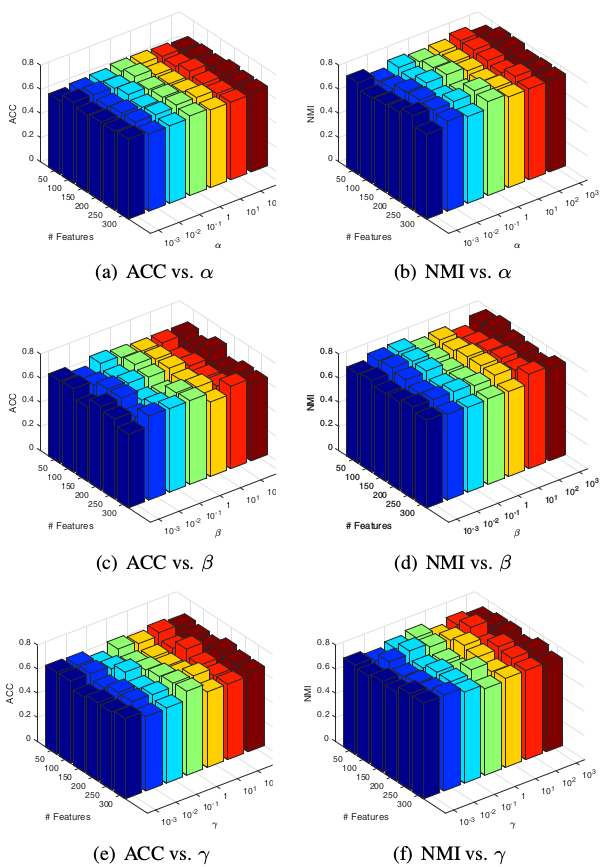
\includegraphics[width=0.8\linewidth]{result_bar.jpg}
\vspace{-8pt}
\captionof{figure}{Performance of JGUFS algorithm for large variation of set of control parameters.}
\end{center}

%------------------------------------------------
\vspace{-15pt}
\begin{center}
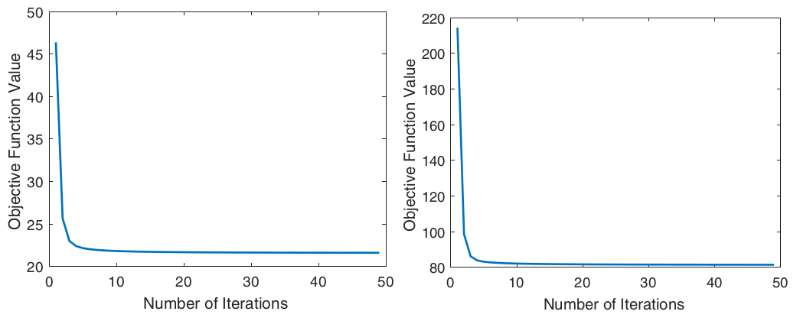
\includegraphics[width=0.8\linewidth]{result_cur.jpg}
\vspace{-8pt}
\captionof{figure}{Convergence speed of JGUFS for UMIST and COIL20 data sets.}
\end{center}

%------------------------------------------------
\vspace{-8pt}
 Figure 2 shows the convergence curves of the JGUFS objective function in terms of the number of iterations on UMIST and COIL20 from which we can observe that JGUFS has a relatively fast convergence speed. 


}

\end{poster}

\end{document}